\documentclass[12pt, border=3mm]{standalone}
\usepackage{tikz}
\usepackage{tkz-euclide}

\begin{document}
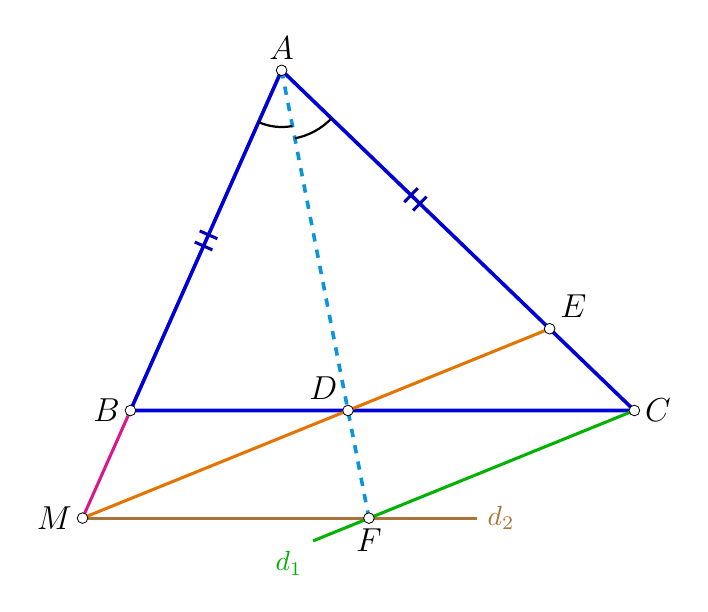
\begin{tikzpicture}[scale=1.6]
    % Tọa độ giải tích chính xác 100%
    \coordinate (A) at (-0.600, 2.700);
    \coordinate (B) at (-1.800, 0.000);
    \coordinate (C) at (2.200, 0.000);
    \coordinate (D) at (-0.073, 0.000);
    \coordinate (E) at (1.527, 0.649);
    \coordinate (M) at (-2.180, -0.854);
    \coordinate (F) at (0.093, -0.854);
    
    % Điểm kéo dài d1 và d2
    \coordinate (d2_end) at (0.950, -0.854);
    \coordinate (d1_end) at (-0.350, -1.035);
    
    % Định nghĩa kiểu đường nét đậm đà rõ ràng
    \tikzset{
        c_main/.style={thick, color=blue!85!black, line width=1.3pt},
        c_line1/.style={color=green!70!black, line width=1.1pt},
        c_line2/.style={color=brown!90!black, line width=1.1pt},
        c_ext1/.style={color=magenta!90!black, line width=1.1pt},
        c_ext2/.style={color=orange!90!black, line width=1.1pt},
        c_sol/.style={thick, color=cyan!80!blue, line width=1.3pt, dashed}
    }
    
    % Tam giác ABC và các đoạn cơ bản
    \draw[c_main] (A) -- (B) -- (C) -- cycle;
    \draw[c_ext1] (B) -- (M);
    \draw[c_ext2] (E) -- (M);
    \draw[c_sol] (A) -- (F); % Đường thẳng đi qua A, D, F
    
    % Đường d2 (qua M và F)
    \draw[c_line2] (M) -- (d2_end) node[right, font=\normalsize] {$d_2$};
    
    % Đường d1 (qua C và F)
    \draw[c_line1] (C) -- (d1_end) node[below left, font=\normalsize] {$d_1$};
    
    % Đánh dấu 2 góc phân giác bằng nhau tại A
    \tkzMarkAngles[size=0.45, arc=l, color=black, line width=0.8pt](B,A,D)
    \tkzMarkAngles[size=0.55, arc=l, color=black, line width=0.8pt](D,A,C)
    
    % Đánh dấu 2 đoạn bằng nhau AB = AE
    \tkzMarkSegments[mark=||, size=3.5pt, color=blue!70!black, line width=1.1pt](A,B A,E)
    
    % Các điểm chấm tròn theo phong cách mẫu
    \foreach \p in {A,B,C,D,E,M,F} {
        \filldraw[fill=white, draw=black, line width=0.3pt] (\p) circle (1.2pt);
    }
    
    % Nhãn đỉnh font toán Computer Modern to rõ
    \tkzLabelPoint[above, font=\large](A){$A$}
    \tkzLabelPoint[left, font=\large](B){$B$}
    \tkzLabelPoint[right, font=\large](C){$C$}
    \tkzLabelPoint[above left, font=\large](D){$D$}
    \tkzLabelPoint[above right, font=\large](E){$E$}
    \tkzLabelPoint[left, font=\large](M){$M$}
    \tkzLabelPoint[below, font=\large](F){$F$}
\end{tikzpicture}
\end{document}
